\section{Ziel}
Das Ziel dieses Versuchs ist es die Strahlendosis und die
Strahlungsleistung in einem mit Röntgenstrahlung bestrahlten
Luftvolumen zu bestimmen.

\section{Theorie}
\label{sec:Theorie}

Die Dosimetrie ist die Lehre von den Verfahren zur Messung 
der von einem System aufgenommenen Dosis bzw. Dosisleistung.
Es wird die mit der ionisierenden Strahlung
verbundene Strahlenwirkung gemessen.


\subsection{Ionendosis J und Ionendosisrate j}
Mit der Ionisation des bestrahlten Materials geht zumeist
eine Absorption von Röntgenstrahlung einher. %gleiche Formulierung wie in der Anleitung
Die Ionendosis ist durch die in Luft erzeugte Ladung $\text{d}Q$
relativ zur Masse $\text{d}m_\text{L}$ der bestrahlten Luft definiert:
\begin{equation*}
    J = \frac{\text{d}Q}{\text{d}m_\text{L}}.
    \label{eqn:Ionendosis}
\end{equation*}

\noindent Die Ionendosisrate $\dot{J}$ entspricht dem zeitlichen Differential der Ionendosis $J$, also gilt 
\begin{equation}
    j = \dot{J} =\frac{\text{d}Q}{dt} \frac{1}{\text{d}m_\text{L}} =\frac{I}{\text{d}m_\text{L}}.
    \label{eqn:Ionendosisrate}
\end{equation}

\subsection{Energiedosis D und die mittlere Energiedosisrate d}
Die Energiedosis ist das Verhältnis von absorbierter
Energie $dE$ zu der Masse $dm$ des Absorbers.
Sie wird beschrieben durch
\begin{equation*}
    D = \frac{\text{d}E}{\text{d}m} = \frac{1}{\rho} \cdot \frac{\text{d}E}{\text{d}V}.
    \label{eqn:Energiedosis}
\end{equation*}
Dabei ist $\rho$ die Dichte des Absorbers.

\noindent Die Energiedosisrate $\dot{D}$ ergibt sich im Mittel zu 
\begin{equation}
    d = \dot{D}_\text{m} = \frac{D}{t} =\frac{E}{m \cdot t} = n \cdot \Phi = \frac{j \cdot \Phi}{e}.
    \label{eqn:Energiedosisrate}
\end{equation}
Dabei ist $\Phi$ die Ionisationsenergie, $n$ die Anzahl der Ionen pro Kilogramm und pro Sekunde. 
Diese ergibt sich zu
\begin{equation*}
    n = \frac{j}{e},
    \label{eqn:Ionenanzahl}
\end{equation*}
wobei $e$ der Elementarladung entspricht. 

\subsection{Äquivalenzdosis H}
Die Wirkung ionisierender Strahlung auf biologische Materie
hängt bei gleicher Energiedosis von der Art der ionisierenden
Strahlung ab. Dieser Einfluss der Strahlungsenergie und -art
auf die biologische Wirkung wird durch den Qualitätsfaktor,
den Faktor der relativen biologischen Wirkung,
beschrieben.
Die Äquivalenzdosis $H$ kann durch diesen Qualitätsfaktor
berechnet werden:
\begin{equation*}
    H = Q \cdot \frac{\text{d}E}{\text{d}m} = Q \cdot D.
    \label{eqn:Aequivalenzdosis}
\end{equation*}

\subsection{Dosisleistung}
Die Dosisleistung ist jeweils die Dosis pro Zeiteinheit.
Kurven gleicher Dosisleistung sind sogenannte Isodosen.

\subsection{Bestrahlung eines Luftvolumens mit Röntgenstrahlung}
Wird ein Luftvolumen in einem Plattenkondensator
(siehe Abb. \ref{fig:Strahlgeometrie}) mit
Röntgenstrahlung bestrahlt und ionisiert, erzeugen die durch
den Röntgenstrahl erzeugten Ionen und Elektronen einen Strom.
Dieser Strom wächst mit steigender Kondensatorspannung 
$U_\text{K}$ an bis er den Sättigungsstrom $I_\text{S}$
erreicht. Mithilfe dieses Stroms können die dosimetrischen
Größen bestimmt werden.
\newline
Das ionisierte Luftvolumen kann folgendermaßen bestimmt werden:
\begin{equation*}
    V = \frac{1}{3} \pi (R^2 (x_0 + x_1 + x_2) - r^2 (x_0 + x_1)). 
\end{equation*}
Dabei sind die Radien
\begin{align*}
    R &= \frac{\text{d} \, x_2}{2 \, x_0} \\
    r &= \frac{\text{d} \, x_1}{2 \, x_0}. 
\end{align*}
Das Volumen ist also 
\begin{equation}
    V = \frac{1}{3} \pi \left(\frac{d^2 x_2^2}{4 x_0^2}(x_0 + x_1 + x_2) - \frac{d^2 x_1^2}{4 x_0^2}(x_0 + x_1)\right).
    \label{eqn:V}
\end{equation}

\begin{figure}
    \centering
    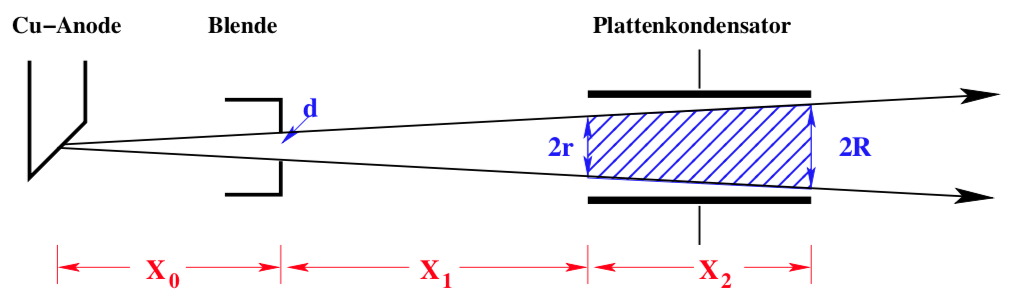
\includegraphics[width=12cm, height=4cm]{build/strahl.png}
    \caption{Es wird die Skizze der Apparatur und ein Strahlengang dargestellt.Links ist eine $Cu$-Anode, in der Mitte eine Blende und rechts ein Plattenkondensator zu sehen. Außerdem ist das bestrahlte Luftvolumen zwischen den Platten des Kondensators blau gekennzeichnet. Die Abstände zwischen den drei Objekten sind unter der Skizze eingezeichnet.\cite{V607}}
    \label{fig:Strahlgeometrie}
\end{figure}

\subsection{Ausgleichsrechnung}

Die Formel für die lineare Regression ergibt sich zu 

\begin{equation}
    y = a \cdot x + b.
    \label{eqn:linreg}
\end{equation}

\noindent Dabei ist $a$ die Steigung und $b$ der $y$-Achsenabschnitt.

\noindent Für die Ausgleichsrechnung einer quadratischen Funktion wird die Formel 
\begin{equation}
    y = a \cdot x^2 + b
    \label{eqn:quadreg}
\end{equation}
benutzt.
Dabei ist $a$ die Amplitude bzw. Stauchung/Streckung und $b$ der $y$-Achsenabschnitt.
